\section{Improving the Multiplexer and Mixed Signal Support}
\label{sec:improving}

Tiny Tapeout 5 split the multiplexer into two parts in order to improve performance. As a result of the split the controller was also updated to multiplex between the two halves.
Some other small changes to the multiplexer include the tweaking, addition, or removal of buffers to improve the STA results.

As each spine segment in Tiny Tapeout 5 is now half as long as in Tiny Tapeout 4, it will exhibit half the capacitance. As a result, we expect to see the round trip latency reduced to around \qty{10}{\ns}.

For Tiny Tapeout 6 the Caravel harness will be replaced by OpenFrame~\cite{openframe}, an alternative harness provided by Efabless that uses the same padring but removes the RISC-V coprocessor.
This results in an additional \qty{5}{\mm\squared} of space for user designs, and 12 more IO pins which will be used for analog signals.

For increased safety, all designs will be power-gated. This allows designers to take more risks in their submissions, or to use custom flows not previously used in Tiny Tapeout.

Analog and mixed signal designs will be enabled by adding an analog multiplexer based on transmission gates~\cite{transmissiongates}. 
This allows up to 192 designs to share the analog pins between them.
These transmission gates were tested as part of an experimental analog submission to Tiny Tapeout 5, shown in Fig.~\ref{fig:transmission_gate_TT05}.

Noise coupling between analog and digital power domains is a known concern. However, due to other limitations of our current setup including its limited number of low bandwidth analog interfaces, we target educational low to medium performance analog and mixed signal designs where noise coupling is a lesser concern.

\begin{figure}[!t]
\centering
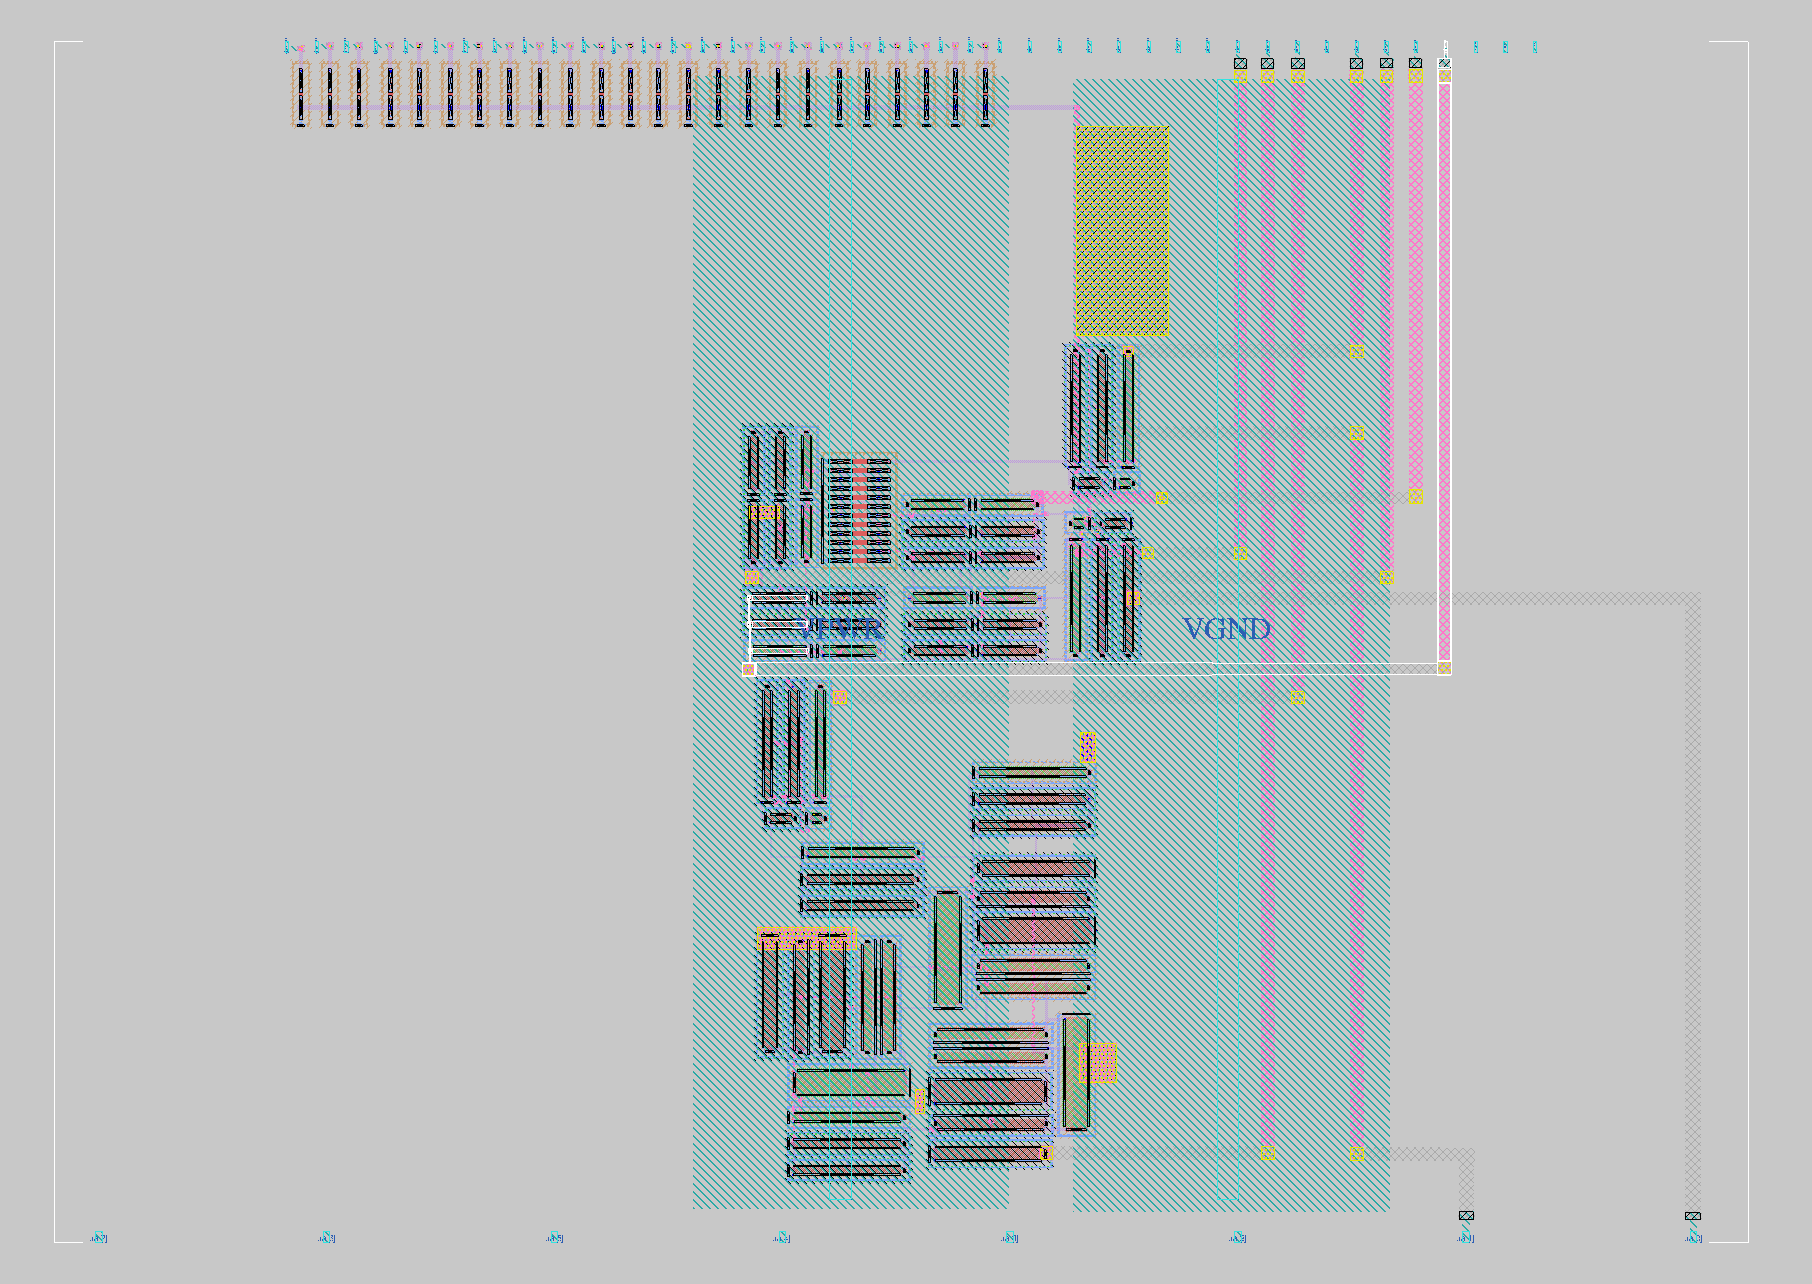
\includegraphics[width=\columnwidth]{./Figs/tt05_transmission_gate.png}
\caption{A ring oscillator and digital to analog converter (DAC) design submitted to Tiny Tapeout 5, with a transmission gate highlighted. This design was automatically placed and routed using an experimental analog place and route (P\&R) tool).}
\label{fig:transmission_gate_TT05}
\end{figure}

Tiny Tapeout 6 is planned to open for submission of digital designs at the end of January 2024, for analog designs at the end of February 2024, and to close for submissions on 19 April 2024.
